\noindent Optische Interferometer zeigen eine starke Abhängigkeit von der Umgebung, in
welcher sie eingesetzt werden. Bereits kleine Erschütterungen des Versuchsaufbaus
können dazu führen, dass sich optische Instrumente mechanisch verstellen und eine
erneute Justage erforderlich machen. \\
\noindent Ein Aufbau des Interferometers nach Sagnac kann bauartbedingt den
Einfluss mechanischer Erschütterungen auf die Stabilität des Versuchsaufbaus
verringern. Grund hierfür ist die Anordnung der Spiegel, von denen jeder die
interferierenden Lichtstrahlen ablenkt, sodass Änderungen des Lichtwegs direkt
in beiden Lichtstrahlen auftreten und daher die Messung relativ betrachtet nicht
stören. \\
\subsection{Das Sagnac-Interferometer}
\noindent Als Interferenz wird die Überlagerung von kohärenten Teilwellen
bezeichnet. Eine Möglichkeit zur Erzeugung solcher Interferenzen ist das
Aufteilen einer von einer Quelle ausgehenden Welle in zwei oder mehrere
Teilwellen, welche unterschiedliche Lichtwege zurücklegen, bevor sie wieder
auf einem Detektor zusammenlaufen. \\
\FloatBarrier
\begin{figure}
  \centering
  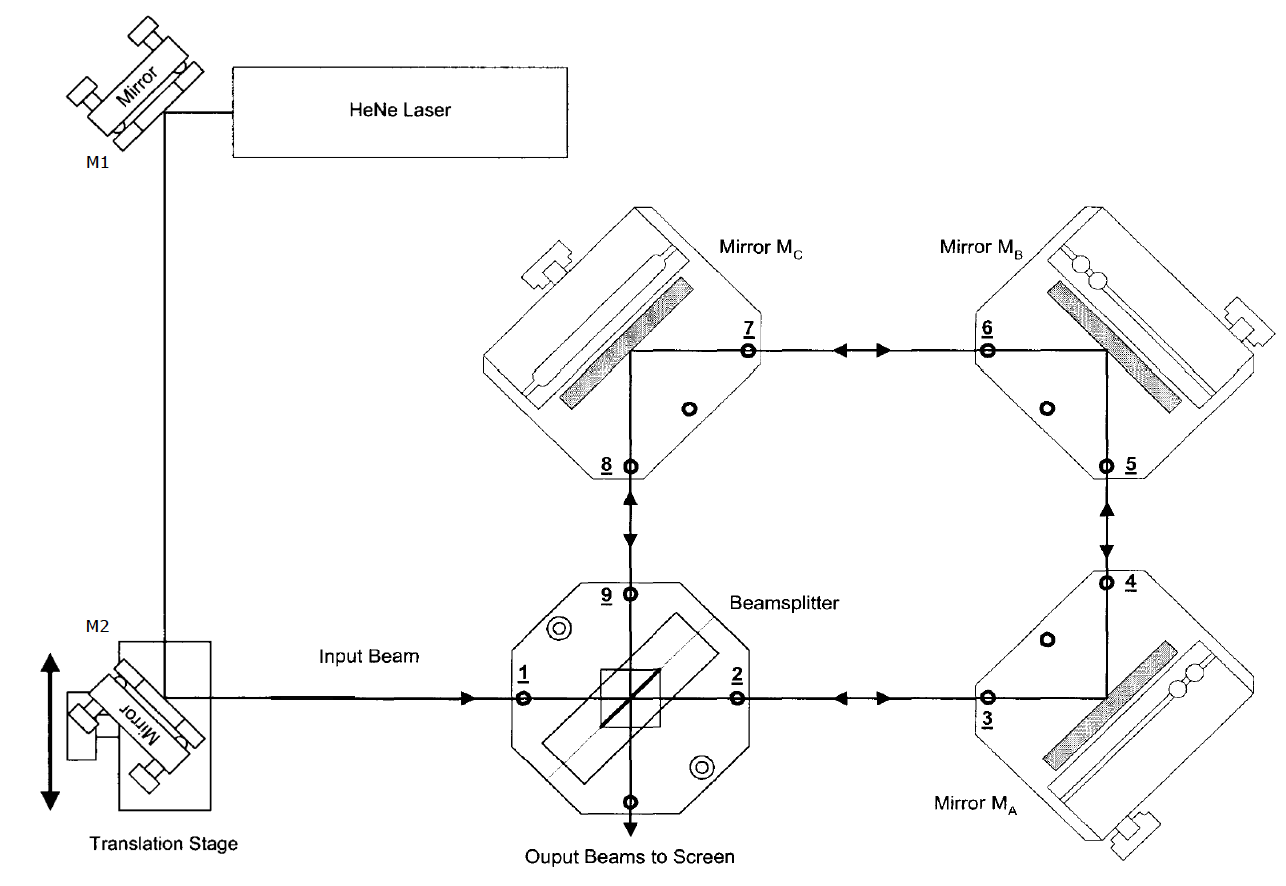
\includegraphics[scale=0.5]{resources/fig_01.png}
  \caption{Schematischer Aufbau eines Sagnac-Interferometers \cite{sample}}
  \label{fig:01}
\end{figure}
\FloatBarrier
\noindent Dieses Prinzip der Lichtaufspaltung wird auch mit dem in Abbildung
\ref{fig:01} dargestellten Sagnac-Interferometer angewandt, allerdings wird
der Lichtweg hier nicht mechanisch durch Veränderung der Positionen der
Umlenkspiegel erreicht, sondern durch eine räumliche Trennung der parallel
verlaufenden Strahlen, von denen ein Strahl durch ein brechendes Medium geführt
wird. Der genaue Strahlengang durch das Sagnac-Interferometer wird im Abschnitt
\ref{durchfuehrung} beschrieben. Dadurch dass das Licht in gegenläufigen
Richtungen exakt die gleichen Bauteile passiert, ist das Sagnac-Interferometer
unanfälliger gegenüber mechanischen Störungen als andere Interferometer. Wird
einer der Spiegel bewegt, so zeichnet sich diese Bewegung in beiden Teilstrahlen
ab, sodass effektiv keine Störung vorliegt. \\
\noindent Um deutliche Intensitätsunterschiede zwischen konstruktiver Interferenz
(Intentensitätsmaximum) und destruktiver Interferenz (Intensitätsminimum) zu
registrieren, ist ein Kontrastwert nahe $K = 1$ zu erzielen. Dieser berechnet
sich über die Gleichung
\begin{align}
  K = \frac{I_\text{max.}- I_\text{min.}}{I_\text{max.} + I_\text{min.}}
  \label{eqn:01}
\end{align}
\noindent und wird nähert sich dem Kontrastmaximum, je schwächer das
Intensitätsminimum ist. \\
\noindent Allgemein lässt sich der Zusammenhang zwischen Strahlungsintensität
und Energie der Lichtwelle für konstante Bestrahlungsstärken vereinfachen zu
\begin{align}
  I = \langle E^2 \rangle,
  \label{eqn:02}
\end{align}
\noindent wobei $E$ die Energie der Lichtwelle beschreibt. Für
\begin{align}
  E(\Theta, t) = E_0 \cdot \cos(\Theta - \omega t)
  \label{eqn:03}
\end{align}
\noindent gilt nach Anwendung des Additionstheorems für Differenzen innerhalb der
Kosinusfunktion
\begin{align}
  E(\Theta, t) = E_0 \cdot \left[\cos(\Theta) \cos(\omega t) + \sin(\Theta) \sin(\omega t) \right].
  \label{eqn:04}
\end{align}
\noindent Durch Wahl einer Phasenverschiebung $\Delta \varphi$ lässt sich
$\sin(\omega t)$ umschreiben zu $\cos(\omega t + \varphi)$. Für die Intensität
des interferierenden Laserlichts gilt für die Energien $E_1$ und $E_2$ damit
der Zusammenhang
\begin{align}
  I = \langle | E_1 \cdot \cos(\Theta) \cos(\omega t) + E_2 \cdot \sin(\Theta) \sin(\omega t) |^2 \rangle.
  \label{eqn:05}
\end{align}
\noindent Aus Gleichung \ref{eqn:05} lässt sich daher auch eine Bedingung für
das Auftreten der Interferenzminima und -maxima ableiten. Das Maximum wird
erreicht, sofern sich die Maximalenergien addieren, das Minima im Falle der
Subtraktion gleich großer Energien, abhängig vpn der Phasenverschiebung $\Delta
\varphi$. Für das Auftreten von Maxima ist folglich eine Phasenverschiebung von
\begin{align*}
  \Delta \varphi_\text{max.} = 2 \cdot \pi \cdot m, \qquad m \in \symbb{N},
\end{align*}
\noindent und für das Auftreten von Minima eine Phasenverschiebung
\begin{align*}
  \Delta \varphi_\text{max.} = (2 \cdot m + 1) \cdot \pi, \qquad m \in \symbb{N},
\end{align*}
\noindent erforderlich \cite{hecht}. Damit lässt sich für Interferenzmaxima und
Interferenzminima Gleichung \ref{eqn:05} schreiben als
\begin{align}
  I_{\frac{\text{max.}}{\text{min.}}} \propto I_\text{Laser} \left[1 \pm 2 \cdot \cos(\Theta) \sin(\Theta) \right].
  \label{eqn:06}
\end{align}
\noindent Der Faktor $I_\text{Laser}$ beschreibt dabei die mittlere
Ausgangsintensität des Lasers und es gilt $I_\text{Laser} \propto (E_1 + E_2)^2$.
Für den Kontrast bedeutet dies unter Berücksichtigung eines Additionstheorems
für trigonometrische Funktionen nach Gleichung \ref{eqn:01} einen Kontrast
\begin{align}
  K \propto | \sin(2 \Theta) |,
  \label{eqn:01b}
\end{align}
\noindent wobei die Maximal- und Minimalwerte nach Gleichung \ref{eqn:06}
bestimmt werden.
\subsection{Brechungsindex von Glas}
\noindent Mithilfe der Anzahl der Interferenzmaxima bzw. Interfernzminima, die
bei der Drehung des Glases durchlaufen werden, lässt sich der Brechungsindex des
Glases bestimmen. Die Anzahl $M$ der Interferenzmaxima lässt sich dabei über die
Gleichung
\begin{align}
  M = \frac{\Delta \varphi}{2 \pi}
  \label{eqn:07}
\end{align}
\noindent bestimmen. Im experimentellen Aufbau werden zwei Glasplättchen von den
Laserstrahlen durchquert. Die Glasplättchen besitzen jeweils eine Dicke $T$ und
sind im Winkel $\alpha = \pm \SI{10}{\degree}$ gegeneinander verkippt. Die
Gleichung für eine einzelne planparallele Platte
\begin{align}
  \Delta \varphi = \frac{2 \pi}{\lambda} \cdot T \cdot \left(\frac{n-1}{2n} \cdot \Theta^2 + O(\Theta^4)  \right)
  \label{eqn:08}
\end{align}
\noindent ist daher noch um die Verkippung zu modifizieren. Werden
Effekte höherer Ordnung, die sich bei der Taylor-Entwicklung in Gleichung
\ref{eqn:08} zeigen vernachlässigt, lässt sich diese schreiben als
\begin{align}
  \Delta \varphi = \frac{2 \pi}{\lambda} \cdot T \cdot \left(\frac{n-1}{2n} \cdot \Theta^2  \right).
  \label{eqn:09}
\end{align}
\noindent Zusammen mit Gleichung \ref{eqn:07} lässt sich daraus die Relation
\begin{align}
  M = \frac{T}{\lambda} \cdot \left( \frac{n-1}{2n} \cdot \Theta^2  \right).
  \label{eqn:10}
\end{align}
\subsection{Brechungsindex von Gasen}
\noindent Neben optisch transparenten Medien wie beispielsweise Glas erfahren
Lichtstrahlen auch in Bereichen verschiedener Umgebungsdrücke Brechung.
Innerhalb der Gaszelle erfährt ein Lichtstrahl eine Phasenverschiebung
\begin{align}
  \Delta \varphi = \frac{2 \pi}{\lambda} \cdot (n - 1) \cdot L,
  \label{eqn:11}
\end{align}
\noindent wobei $L$ der Länge der Gaszelle entspricht. Unter Berücksichtigung
von Gleichung \ref{eqn:07} ergibt sich daraus der Zusammenhang
\begin{align}
  M = \frac{n-1}{\lambda} \cdot L,
  \label{eqn:12}
\end{align}
\noindent bzw. aufgelöst nach dem Brechungsindex $n$
\begin{align}
  n = \frac{M \cdot \lambda}{L} + 1
  \label{eqn:13}
\end{align}
